\documentclass[a4paper,12pt]{report}
\usepackage{fullpage}
\usepackage{amsmath}
\usepackage{fancyhdr}
\usepackage{lastpage}
\usepackage{chngcntr}
\usepackage{changepage}
\usepackage{graphicx}
\usepackage{lipsum}
\usepackage{color, soul}
\usepackage{tabularx}
\usepackage{listings}
\usepackage{courier}
\usepackage{pgfplots}
\pagestyle{fancy}
\fancyhf{}
\setlength{\headheight}{40pt}
\setlength{\headsep}{0.2in}

\lhead{4-23-2019}
\chead{EECS 649 Homework 10}
\rhead{Cameron Kientz \quad \thepage/\pageref{LastPage}}

\newcounter{problem}
\newenvironment{problem}[2][]{
    \noindent
	% \begin{minipage}{\textwidth}
    \refstepcounter{problem}
    \noindent
    \textbf{\underline{Problem~\theproblem#1}} \bigskip\newline
    \textbf{#2} \bigskip
    \begin{adjustwidth}{1em}{}
    }{\end{adjustwidth}\noindent\rule{\textwidth}{0.4pt}\bigskip
	% \end{minipage}
	}

\newcounter{subproblem}
\counterwithin{subproblem}{problem}
\newenvironment{subproblem}[2][]{
	\begin{minipage}{\textwidth}
    \refstepcounter{subproblem}\textbf{\underline{Part~\alph{subproblem}#1}}
    \textbf{#2} \bigskip
    \begin{adjustwidth}{0.5em}{}
    }{\end{adjustwidth}\bigskip
	\end{minipage}
	}

\lstset{
   basicstyle=\fontsize{8}{5}\selectfont\ttfamily,
   language=Python
}

%%PROBLEM #%%
% \begin{problem}{Questions words?}
%     \begin{subproblem}{Subquestion words}
%         Answer words
%     \end{subproblem}
% \end{problem}

%%PROBLEM #%%
% \begin{problem}{Questions words?}
%     Answer words
% \end{problem}


\begin{document}

%%PROBLEM 1%%
\begin{problem}{Give a decision tree to represent each of the following boolean functions:}
    \begin{subproblem}{A and (not B)}
        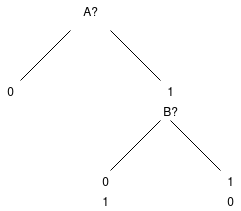
\includegraphics[width=0.3\textwidth]{fig4.png}
    \end{subproblem}
    \begin{subproblem}{A or (B and C)}
         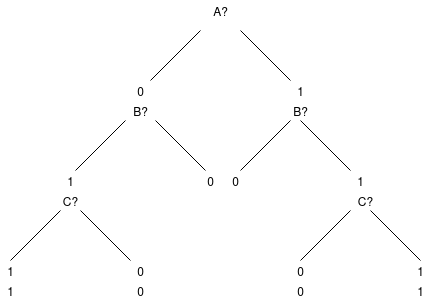
\includegraphics[width=0.3\textwidth]{fig5.png}
    \end{subproblem}
    \begin{subproblem}{A xor B}
        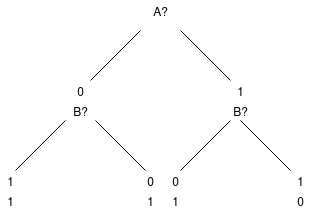
\includegraphics[width=0.3\textwidth]{fig6.png}
    \end{subproblem}
    \begin{subproblem}{(A and B) or (C and D)}
        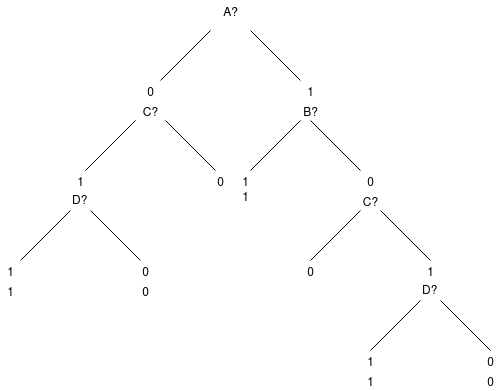
\includegraphics[width=0.3\textwidth]{fig7.png}
    \end{subproblem}
\end{problem}

\newpage

%PROBLEM 2%%
\begin{problem}{Consider this set of training examples: \newline
    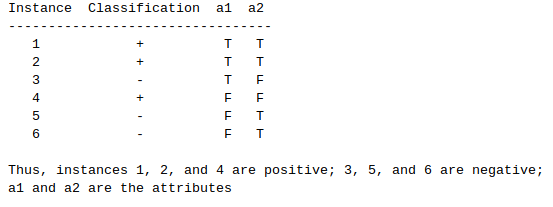
\includegraphics[width=0.6\textwidth]{fig1.png}}
    \begin{subproblem}{What is the entropy of this set of training examples with respect to the target function classification?}
        The entropy of this set is 2 bits, since it takes 2 bits to determine the positive or negative value
    \end{subproblem}
    \begin{subproblem}{What is the information gain of a2 relative to these training examples?}
        The information gain of a2(as well as a1) is 1 bit, since knowledge of a2 reduces the entropy level of 
        the classification by 1 bit.
    \end{subproblem}
\end{problem}

%%PROBLEM 3%%
\begin{problem}{This is a question about the Decision-Tree-Learning Algorithm (aka ID3)}
    \begin{subproblem}{Show the decision tree that would be learned by ID3 assuming it is given the four training 
    examples below for the EnjoySport? target concept.
    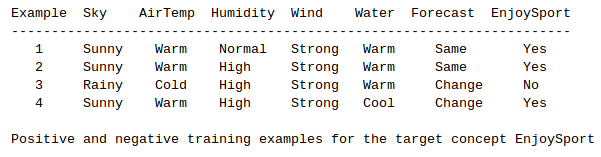
\includegraphics[width=0.6\textwidth]{fig2.png}}
        Answer words
    \end{subproblem}
    \begin{subproblem}{Add the following training example, and compute the new decision tree. This time, show the 
    value of the information gain for each candidate attribute at each step in growing the tree.
    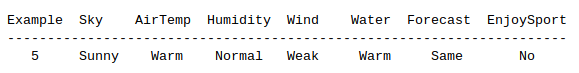
\includegraphics[width=0.6\textwidth]{fig3.png}}
        Answer words
    \end{subproblem}
\end{problem}

%%PROBLEM 4%%
\begin{problem}{Consider  an  ensemble  learning  algorithm  that  uses  simple  majority  voting  among K learned  hypotheses.
   Suppose that each hypothesis  has error $\epsilon$ and that the errors made by each hypothesis are independent  of the others’.  
   Calculate a formula for the error of the ensemble algorithm in terms of K and $\epsilon$, and evaluate it for the cases where K=5 and 
   $\epsilon=0.1$.}
    \[Error = \sum_{i=\frac{K+1}{2}}^K \frac{K}{i}\epsilon^i(1-\epsilon)^{K-i}\]
    Therefore the Error comes out to 0.00857
\end{problem}

\newpage

%%PROBLEM 5%%
\begin{problem}{Find and sketch the following, and Report the actual polynomials found, simplifying to a single number each of their coefficients.}
    \begin{subproblem}{1st-order (linear) Lagrange interpolating polynomial through (1,2) and (3,5)}
        \[L(x) = 2*\frac{2(x-3)}{1-2} + 5*\frac{x-1}{3-1} \rightarrow L(x) = \frac{1}{2}x + \frac{7}{2}\]
        \begin{tikzpicture}
            \begin{axis}[ 
                xlabel=$x$,
                ylabel={$L(x) = \frac{1}{2}x + \frac{7}{2}$}
            ] 
                \addplot {0.5*x + 3.5}; 
            \end{axis}
        \end{tikzpicture}
    \end{subproblem}
    \begin{subproblem}{2nd-order (quadratic) Lagrange interpolating polynomial through (-1,0.1), (0,0), (1,0.1)}
        \[L(x) = 0.1*\frac{x(x-1)}{(-1)(-1-1)} + 0 + .1*\frac{x(x-(-1))}{1(1-(-1))} \rightarrow L(x) = 0.05(x^2-x) + 0.05(x^2+x)\]
        \begin{tikzpicture}
            \begin{axis}[ 
                xlabel=$x$,
                ylabel={$L(x) = 0.05(x^2-x) + 0.05(x^2+x)$}
            ] 
                \addplot {0.05(x^2-x) + 0.05(x^2+x)}; 
            \end{axis}
        \end{tikzpicture}
    \end{subproblem}
    \begin{subproblem}{1st-order (linear) least squares fit for points (-1,0.1), (0,0), (1,0.1)}
        Answer words
    \end{subproblem}
\end{problem}

%%PROBLEM 6%%
\begin{problem}{For this problem you will implement code to compute a "decision stump" for a real-life data set
    The data is a massaged version (to make all variables 0-1 valued and remove instances with missing values) of 
    the Congressional Voting Records in the UCI Machine Learning database. There is the classification (Attribute 1; 
    0=Democrat, 1=Republican) and 16 attributes (Attributes 2-17), which details votes on various bills taken from 
    the 1984 United States Congressional Voting Records (0=nay, 1=yes).}
    \begin{subproblem}{Write a subroutine for Remainder(A), described on page 704 of R\&N, that takes as its input value 
    for A an integer between 2 and 17 corresponding to Attributes 2-17 as defined in the data file.}
        Answer words
    \end{subproblem}
    \begin{subproblem}{Write a subroutine for Gain(A), again described on page 704 of R\&N, that again takes an integer 
    input as above.}
        Answer words
    \end{subproblem}
    \begin{subproblem}{Write the necessary code to compute the decision stump. This entails (i) finding the attribute (2-17) 
    that maximizes the information gain, (ii) counting how many of each classification appear in each branch, and (iii) computing 
    the classifications you should use depending on that attribute's value.  So, you are splitting on the yeses and nays (for 
    each vote) and trying to predict the Dems and Reps. IDEA: how can you best predict the rep.’s party by their vote on just one 
    particular bill?}
        Answer words
    \end{subproblem}
\end{problem}

\end{document}
